
%\begin{IEEEbiography}[{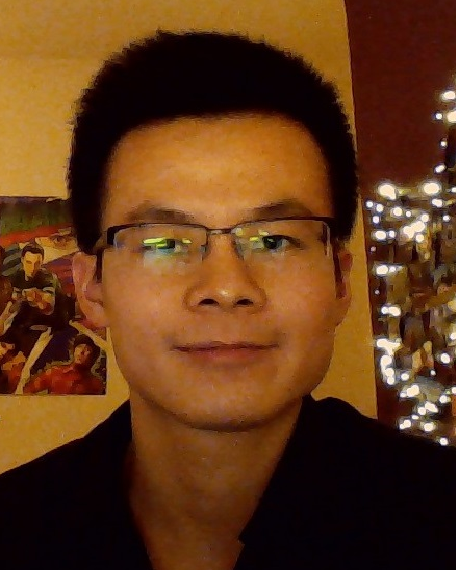
\includegraphics[width=1in,height=1.25in,clip,keepaspectratio]{images/biography/dwu_s}}]{Di Wu}
%Biography text here.
%\end{IEEEbiography}


\begin{IEEEbiography}[{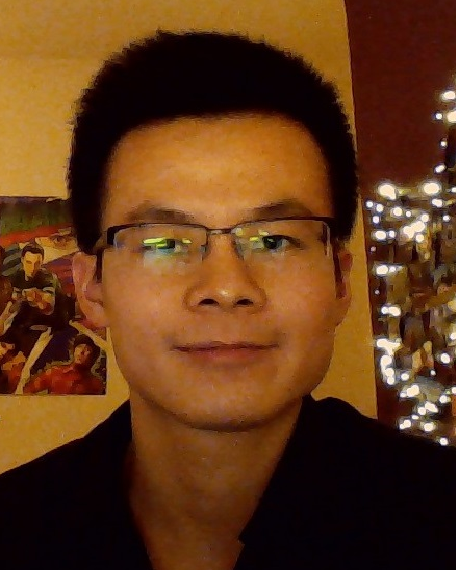
\includegraphics[width=1in,height=1.25in,clip,keepaspectratio]{images/biography/dwu_s}}]{Di Wu}
received his Bachelor degree from Zhejiang University in 2010 and his PhD degree from the University of Sheffield in 2014. He is currently a postdoctoral researcher at the Idiap Research Institute. His research interests include using machine learning techniques, such as probabilistic graphical models and deep learning for high-level computer vision tasks, such as human action recognition, gesture recognition, medical images analysis, person identification and multimedia retrieval.
\end{IEEEbiography}

\begin{IEEEbiography}[{\includegraphics[width=1in,height=1.25in,clip,keepaspectratio]{images/biography/LP004.jpg}}]{Lionel Pigou}
received a M.Sc. degree in computer science at Ghent University in 2014, where he is currently pursuing a Ph.D. in machine learning. His research interests are focused on deep learning and how it can be applied on gesture and sign language recognition in spatiotemporal data.
\end{IEEEbiography}


\begin{IEEEbiography}[{\includegraphics[width=1in,height=1.25in,clip,keepaspectratio]{images/biography/PJK.jpg}}]{Pieter-Jan Kindermans}
obtained his Bachelor degree in Informatics (2008) and his Master degree in Computer Science Engineering (2010) at Ghent University, Belgium. In 2014 he finished his PhD in Computer Science in Ghent. Currently he has a postdoc position as a Marie Curie fellow in the machine learning group at TU-Berlin.
\end{IEEEbiography}


\begin{IEEEbiography}[{\includegraphics[width=1in,height=1.25in,clip,keepaspectratio]{images/biography/namle.jpg}}]{Nam Do-Hoang Le}
 obtained his Bachelor's degree and Master's degree in computer science from the University of Science, Hochiminh, Vietnam in 2012 and 2014 respectively. 
He is currently pursuing the Ph.D. degree at the Idiap Research Institute, Martigny, Switzerland, and \'Ecole Polytechnique F\'ed\'erale de Lausanne, Lausanne, Switzerland.
\end{IEEEbiography}


\begin{IEEEbiography}[{\includegraphics[width=1in,height=1.25in,clip,keepaspectratio]{images/biography/Ling_Shao.jpg}}]{Ling Shao}
(M'09-SM'10) is a Full Professor and Head of the Computer Vision and Artificial Intelligence Group with the Department of Computer Science and Digital Technologies at Northumbria University, Newcastle upon Tyne and an Advanced Visiting Fellow with the Department of Electronic and Electrical Engineering at the University of Sheffield. Previously, he was a Senior Lecturer (2009-2014) with the Department of Electronic and Electrical Engineering at the University of Sheffield and a Senior Scientist (2005-2009) with Philips Research, The Netherlands. His research interests include Computer Vision, Image/Video Processing, Pattern Recognition and Machine Learning. He is an Associate Editor of IEEE Transactions on Neural Networks and Learning Systems, IEEE Transactions on Image Processing, IEEE Transactions on Circuits and Systems for Video Technology, and several other journals.  He is a Fellow of the British Computer Society and a Fellow of the IET.
\end{IEEEbiography}


\begin{IEEEbiographynophoto}{ Joni Dambre}
is a Professor at Ghent University.
\end{IEEEbiographynophoto}

\begin{IEEEbiography}[{\includegraphics[width=1in,height=1.25in,clip,keepaspectratio]{images/biography/odobez.jpg}}]{Jean-Marc Odobez}
(\'Ecole Nationale Sup\'erieure de T\'el\'ecommunications de Bretagne (ENSTBr), France, 1990;
PhD at INRIA, Rennes University, France, 1994),
was associate professor in computer science at the  Universit\'e du Maine, Le Mans, France, from 1996 to 2001.
He is now a senior researcher at both the Idiap Research Institute and
EPFL, Switzerland, where he directs the Perception and Activity Understanding group.
His main areas of research are computer vision and machine learning
techniques applied to multimedia content analysis, tracking,
and human activity and behavior recognition. He is the author or
coauthor of more than 120 papers in international journals and
conferences. He is or was the principal investigator of 10
European and Swiss projects. He holds two patents on video motion
analysis. He is the cofounder of the Swiss Klewel SA company active in
the intelligent capture, indexing of multimedia events. He is a member of the IEEE, and associate
editor of the IEEE Transaction on Circuits and Systems for Video Technology and Machine Vision and Application journals.
\end{IEEEbiography}


% insert where needed to balance the two columns on the last page with
% biographies
%\newpage

% You can push biographies down or up by placing
% a \vfill before or after them. The appropriate
% use of \vfill depends on what kind of text is
% on the last page and whether or not the columns
% are being equalized.

%\vfill

% Can be used to pull up biographies so that the bottom of the last one
% is flush with the other column.
%\enlargethispage{-5in}
\endinput
